\documentclass[english,a4paper,10pt]{scrartcl}

\usepackage[left=2.5cm,right=2.5cm,top=2.5cm,bottom=2cm,includefoot]{geometry}

\usepackage[utf8]{inputenc}
\usepackage[T1]{fontenc}

\usepackage{natbib}
\usepackage{graphicx}
\usepackage{multirow}
\usepackage{amsmath,amssymb,amsfonts}
\usepackage{textcomp}
\usepackage{manyfoot}
\usepackage{listings}
\usepackage{booktabs}
\usepackage[section]{placeins}

\graphicspath{{gfx/}}
\newcommand{\degr}[1]{\text{\textdegree #1}}

\usepackage{babel}
\usepackage{stmaryrd}

\usepackage[colorlinks=true,allcolors=blue]{hyperref}
\hypersetup{bookmarksdepth=3}

\begin{document}

\title{Report\\[2ex] Seasonal-level prediction in African countries for agricultural production risk assessment}

\author{Andreas Groth}
\date{July 1, 2023}

\maketitle

\section{Introduction}

\subsection{General background}

Understanding of the features and drivers of natural climate variability or of the response of the climate system to anthropogenic greenhouse gases forcing are needed for risk and impact studies across ecosystems and society. The development of Earth Systems Models (ESMs) has underlined much of the research in climate sciences to understand and predict the evolution of climate variability since the mid 1970s with \citet{Manabe.Bryan.ea.1975} pioneering work. ESMs have been used to study the dynamics of sub-seasonal, to annual and decadal climate variability \citep{Robertson.Vitart.ea.2020} -- for instance to assess how sea surface temperature (SST) anomalies may affect surface air temperature multiscale spatial and temporal variability, or how decadal variability responds to anthropogenic greenhouse forcing.

The operational predictions used by the climate research community rely on multi-model ensembles. For instance, the Copernicus Climate Change Services \citep{C3S} provides sub-seasonal to seasonal forecasts up to six months ahead and the North American Multi-Model Ensemble \citep{NMME} provides forecasts for up to 12 months.

Recently, machine learning and neural network-based techniques have been suggested in this field to understand and forecast low to high-frequency climate processes. The emergence of physically constrained machine-learning-techniques has in particular shown promise to generalize beyond the training data used \citep{Irrgang.Boers.ea.2021,Kashinath.Mustafa.ea.2021}.

In this report, we propose the application of a methodological approach based on a a variational auto-encoder (VAE) introduced in \cite{Groth.Chavez.2023} for the prediction of rainfall variability in Africa. For an accompanying  application to the decadal prediction subject to different Greenhouse Gas emission scenario, we refer to \cite{Groth.SSP.2023}.

The VAE is a universal, state-of-the-art neural network (NN)-based machine learning approach \citep{Kingma.Welling.2014} that is not limited to any specific kind of data and allows for representation learning with many applications in computer vision \citep{Higgins.Matthey.ea.2017,Chen.Li.ea.2018,Dosovitskiy.Djolonga.2020}, natural language processing \citep{Bowman.Vilnis.ea.2015} and other fields \citep{Hafner.Lillicrap.ea.2021}. In this report, we rely on the VAE architecture introduced by \cite{Groth.Chavez.2023} that allows to disentangle the complexity inherent to large climate datasets and that helps us extract underlying generic properties shared by an ensemble of ESMs. Here, the underlying objective is to build an ESM emulator that will then be fine-tuned on historical observations of climate variability to provide sub-seasonal to seasonal predictions of rainfall variability in Africa.

\subsection{Subject of the study}

In this report, we focus on Africa precipitation and the seasonal-level prediction in target countries for agricultural production risk assessment. In Southern and Eastern Africa, two major drivers of subseasonal to interannual climate variability are the El Niño Southern Oscillation (ENSO) and the Indian Ocean Dipole (IOD). ENSO is the dominant mode of interannual climate variability in the tropical Pacific Ocean and is characterized by a coupled ocean-atmosphere interaction. The IOD is a coupled ocean-atmosphere phenomenon in the Indian Ocean that is characterized by a dipole pattern of SST anomalies. The IOD and ENSO are known to influence rainfall variability in Southern and Eastern Africa \citep{Kundzewicz.Szwed.ea.2019,Nicholson.2017}, and we propose to combine ENSO and IOD prediction with rainfall prediction for lead times of 6 to 12 month ahead. Achieving the latter will involve to:

\begin{itemize}
    \item Integrate global SST, represented as gridded global SST, as input to a VAE.
    \item Predict global SST and, consequently the ENSO and IOD indices.
    \item Jointly integrate gridded rainfall that covers Southern and Eastern Africa as input to a VAE.
    \item Jointly predict rainfall in Southern and Eastern Africa.
    \item The VAE will be pre-trained on historical runs from CMIP6 and transfer-learned on historical observations.
\end{itemize}

This will allow us to build an interpretable model of rainfall prediction in a sense that we can study the uncertainty in ENSO and IOD prediction jointly with the uncertainty in rainfall prediction and therefore put the prediction into a more physically relevant interpretable context. This approach aims to improve the VAE's ability to predict precipitation in Southern and Eastern Africa by leveraging the knowledge gained from global SST.

The report is organized as follows: In Section~\ref{sec:methodology}, we first give a brief overview of the data used in this study and then present general principles of the VAE and the variant that we propose here. In Section~\ref{sec:model-architecture}, we present further details on the architecture of the NNs used to build the VAE. Section~\ref{app:model-params-training} provides technical details about model configuration and model training and Section~\ref{sec:results} presents the results of the VAE.

\section{Methodology}\label{sec:methodology}

In this section, we first give a brief overview of the data used in this study. Next, we present the general principles of the VAE and discuss more recent variants that improve the learning of disentangled latent factors. Finally, we present the VAE variant of \cite{Groth.Chavez.2023} which combines the auto-encoding objective with a prediction task.

\subsection{Data}\label{sec:data}

The coupled general circulation climate model simulations analyzed in this study are from the sixth phase of the Coupled Model Intercomparison Project \citep[CMIP6,][]{Flynn.Mauritsen.2020}. We use monthly global SST anomalies from historical simulations over the 1850--2014 period . Multiple runs of each of the CMIP6 models are taken and interpolated onto a regular $5\degr{}\times5\degr{}$ global grid between $60\degr{S}$ and $60\degr{N}$.

Furthermore, we use the corresponding monthly global rainfall anomalies from the set of historical simulations, interpolated onto a regular $1\degr{}\times1\degr{}$ global grid covering Southern and Eastern Africa. The region of interest is defined as the area between $35\degr{S}$ and $5\degr{N}$, and $9\degr{E}$ and $50\degr{E}$.

The proposed model uses principal components (PCs) of global SST and rainfall anomalies as input that allows us to infer information on spatiotemporal aspects of ENSO and IOD, and relate them to rainfall anomalies in the region of interest.

For the SST anomalies, a single set of empirical orthogonal functions (EOFs) is computed to identify the leading modes of variability common to all CMIP6 models. For this purpose, the different runs of each model are concatenated before the eigendecomposition. Then, the different runs are projected onto the resulting EOFs to obtain the PCs for each model. In the present work, the leading $S=20$ PCs are used as input to the VAE, capturing about 55\% of the total variance in the ensemble of global SST anomalies.

For the rainfall anomalies, we likewise compute a single set of EOFs from the concatenated rainfall anomalies of all CMIP6 models. The leading $S=20$ EOFs are used as input to the VAE, capturing about 80\% of the total variance in the ensemble of rainfall anomalies.

Furthermore, we use historical observations of monthly global SST data taken from the fifth version of the NOAA Extended Reconstructed Sea Surface Temperature \citep[ERSST,][]{Huang.Thorne.ea.2017.ERSST}. We use SST anomalies over the 1891--2014 period projected onto the CMIP SST EOFs to obtain ERSST PCs. Similarly, we use historical observations of monthly global rainfall data from the Global Precipitation Climatology Centre \citep[GPCC,][]{Schneider.Haensel.ea.2022} over the 1891--2014 period. The GPCP data are projected onto the CMIP rainfall EOFs to obtain GPCC PCs.

\subsection{Variational auto-encoding}
\FloatBarrier
\begin{figure}
    \centering{}
    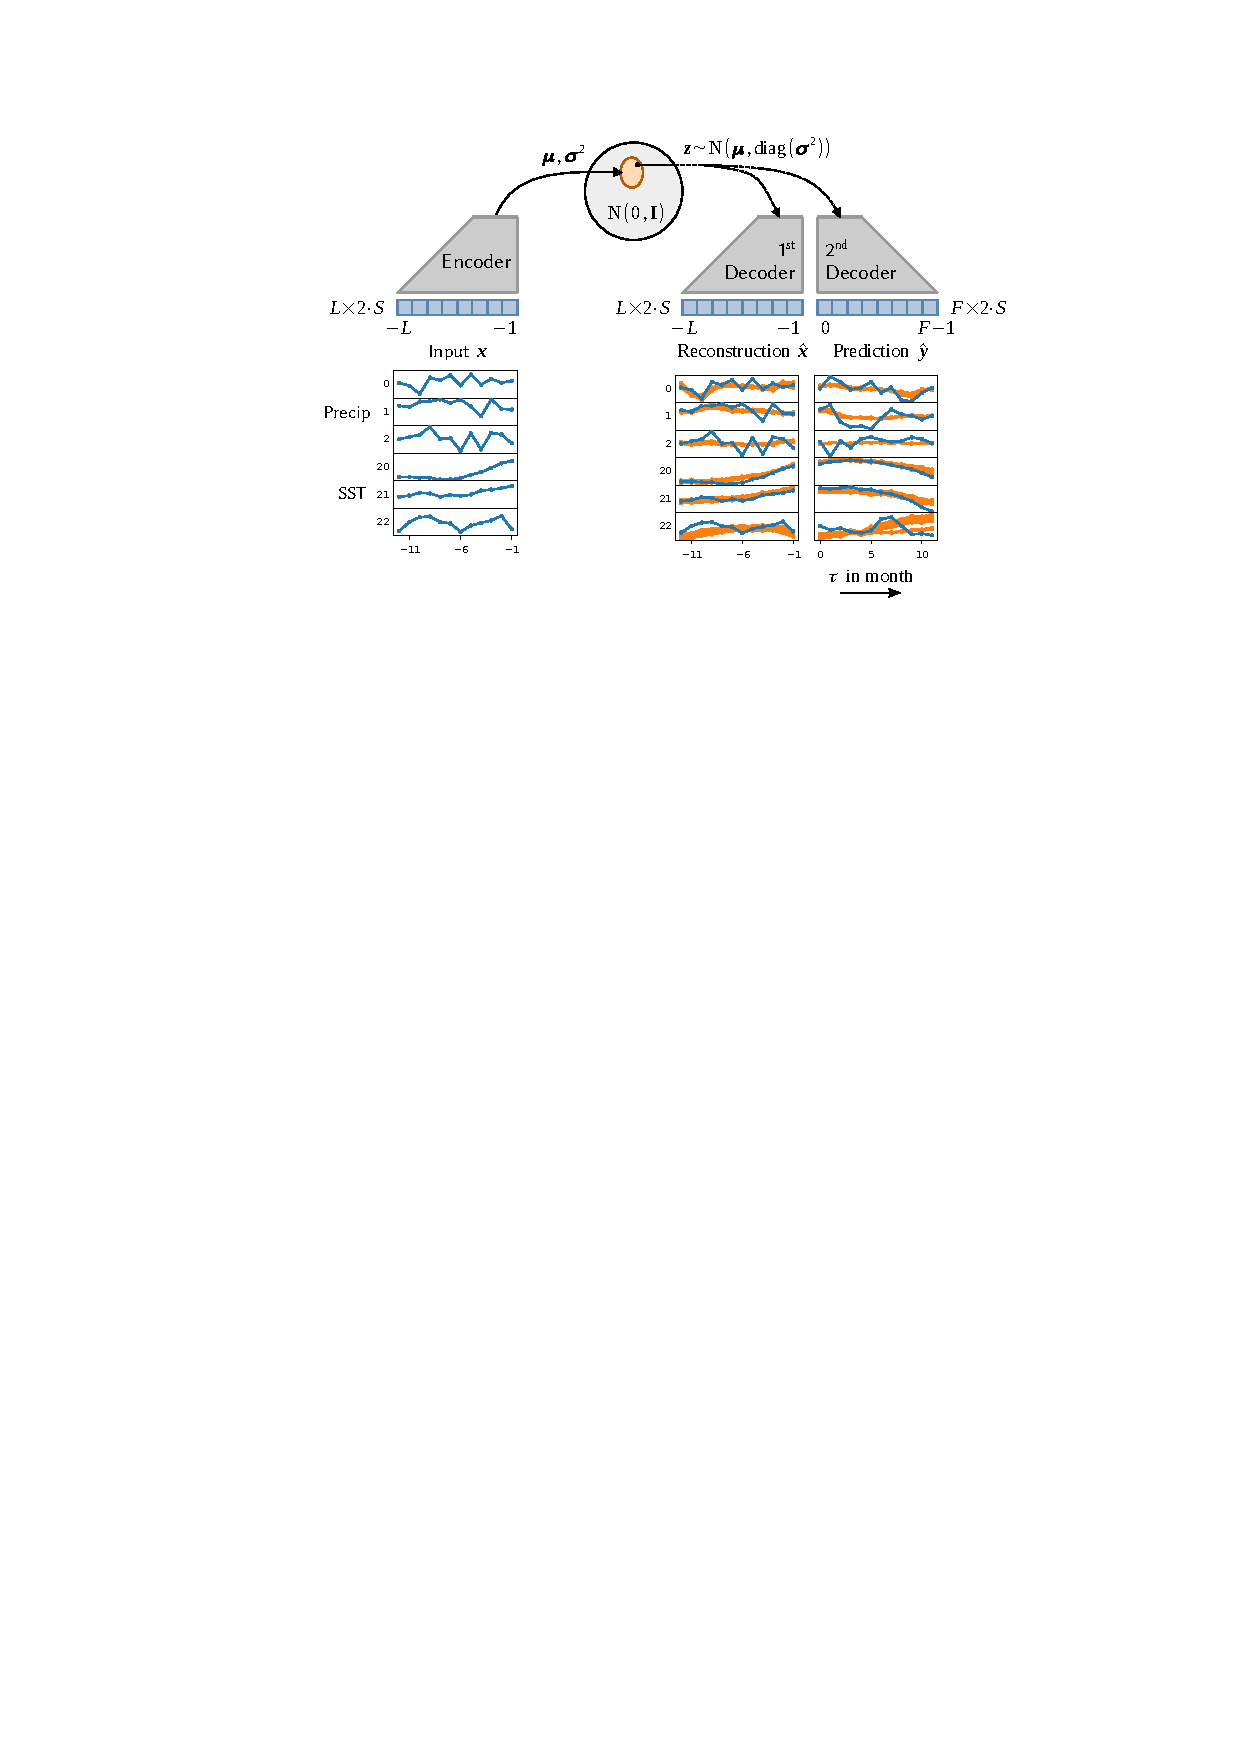
\includegraphics[width=0.8\linewidth]{Fig1_model_overview.pdf}
    \caption{\label{fig:model-overview}
        Overview of the model components. The model is a combination of a VAE, with its encoder (left) and decoder (middle), and a second decoder for prediction (right). An example of the input $\mathbf{x}$ to the encoder (blue) and the resulting stochastic reconstruction $\mathbf{\hat{x}}$ and prediction $\mathbf{\hat{y}}$ (orange) are shown below the corresponding model parts. With a prior $\mathcal{N}(0,\mathbf{I})$ over the latent space, the encoder approximates a posterior $\mathcal{N}(\boldsymbol{\mu},\mathrm{diag}(\boldsymbol{\sigma}^{2}))$, which is used by the two decoders to stochastically estimate the input $\mathbf{x}$ and prediction target $\mathbf{y}$ (blue).}
\end{figure}

The VAE combines variational inference with deep learning and provides a probabilistic approach to describe observations in the latent space \citep{Kingma.Welling.2014,Kingma.Welling.2019}. The VAE encoding and decoding methodology provides a computationally efficient way to a) infer information about latent variables from observations and b) to approximate the difficult-to-compute probability density functions (PDFs) that underlie the complex nonlinear dynamics in the multi-model CMIP ensemble.

To achieve this, the VAE is trained on samples from the multi-model dataset $\mathcal{D}=\{\mathcal{D}_{M}\}_{m=1}^{M}$ that combines the $M$ different historical simulations, $\mathcal{D}_{m}=\{\mathbf{x}_{m}(n)\}_{n=1}^{N}$, each providing $N$ training samples (cf. Fig.~\ref{fig:model-overview}). In the following, we omit the index $m$ when referring to the entire multi-model dataset $\mathcal{D}$.

\paragraph{Auto-encoding}
The encoder $q$, parameterized by a neuronal network (NN) with parameters $\phi$, approximates the PDF of the latent space $\mathbf{z}$ conditional on the sample $\mathbf{x}$,
\begin{equation}
    q_{\phi}(\mathbf{z}|\mathbf{x}).\label{eq:encoder-pdf}
\end{equation}
The decoder $p$, parameterized by a second NN with parameters $\theta$, approximates the PDF of the sample $\mathbf{x}$ conditional on the latent space $\mathbf{z}$,
\begin{equation}
    p_{\theta}(\mathbf{x}|\mathbf{z}).\label{eq:decoder-pdf}
\end{equation}
In jointly optimizing the parameters of the encoder and decoder, the VAE learns to find stochastic mappings between a high-dimensional input space $\mathbf{x}$, whose distribution is typically complicated, and a low-dimensional latent space $\mathbf{z}$, with a distribution that is comparatively much simpler.

\paragraph{Generative model}
The VAE combines an inference model with a generative model. The inference model, represented here by the encoder, approximates the true but difficult-to-compute (intractable) posterior, $p(\mathbf{z}|\mathbf{x})\approx q_{\phi}(\mathbf{z}|\mathbf{x})$. The generative model then learns a joint distribution $p_{\theta}(\mathbf{x},\mathbf{z})$ between input space and latent space, which allows us to continuously generate new unseen data in input space while sampling from the latent space. The generative model is typically factorized as
\begin{equation}
    p_{\theta}(\mathbf{x},\mathbf{z})=p_{\theta}(\mathbf{z})p_{\theta}(\mathbf{x}|\mathbf{z}),\label{eq:generative-model}
\end{equation}
with a prior distribution $p_{\theta}(\mathbf{z})$ over the latent space and the decoder $p_{\theta}(\mathbf{x}|\mathbf{z})$ in Eq.~\eqref{eq:decoder-pdf}. The prior is taken from a family of densities whose parameter can be easily optimized; cf. section~\ref{sec:gaussian-approximation}.

\paragraph{Evidence lower bound}
To improve the generative model in Eq.~\eqref{eq:generative-model}, we maximize the \emph{evidence lower bound} (ELBO),
\begin{subequations}
    \begin{eqnarray}
        \mathcal{L}_{\mathrm{ELBO}}(\mathbf{x}) &=& \mathbb{E}_{q_{\phi}(\mathbf{z}|\mathbf{x})}\left[\log\left(\frac{p_{\theta}(\mathbf{x},\mathbf{z})}{q_{\phi}(\mathbf{z}|\mathbf{x})}\right)\right],\label{eq:ELBO} \\
        &\leq& \log p_{\theta}(\mathbf{x}),
    \end{eqnarray}
\end{subequations}
which puts a lower bound on the log likelihood of the data that we wish to model \citep{Kingma.Welling.2014}. Maximizing Eq.~\eqref{eq:ELBO} jointly optimizes the parameters $\theta$ and $\phi$ of the encoder and decoder, improving at the same time the generative model in its ability to generate more likely (more realistic looking) data, and the inference model in the approximation of the true posterior distribution (of the data-generating factors).

Using Eq.~\eqref{eq:generative-model}, the ELBO in Eq.~\eqref{eq:ELBO} can be rewritten as the sum of two terms,
\begin{subequations}
    \begin{eqnarray}
        \mathcal{L}_{\mathrm{ELBO}}(\mathbf{x}) & = & \mathbb{E}_{q_{\phi}(\mathbf{z}|\mathbf{x})}\left[\log p_{\theta}(\mathbf{x}|\mathbf{z})\right] + \mathbb{E}_{q_{\phi}(\mathbf{z}|\mathbf{x})}\left[\log\left(\frac{p_{\theta}(\mathbf{z})}{q_{\phi}(\mathbf{z}|\mathbf{x})}\right)\right],\\
        & = & \mathbb{E}_{q_{\phi}(\mathbf{z}|\mathbf{x})}\left[\log p_{\theta}(\mathbf{x}|\mathbf{z})\right] - \mathrm{KL}\left(q_{\phi}(\mathbf{z}|\mathbf{x})\Vert p_{\theta}(\mathbf{z})\right),\label{eq:ELBO-components}
    \end{eqnarray}
\end{subequations}
i.e., the sum of a) the expected log-likelihood of the data $\mathbf{x}$, which is a measure of the reconstruction error of the decoder $p_\theta$, and b) the Kulback-Leibler (KL) divergence, which acts as a regularization term on the encoder $q_\phi$.

\subsection{Disentangled representations}

In order to improve the generalization capabilities of the VAE and to learn a more interpretable representation of the data, we wish to learn a representation that is disentangled, i.e., where each latent dimension corresponds to a single generative factor of the data. For this purpose, \cite{Groth.Chavez.2023} propose to add several modifications to the vanilla VAE objective in Eq.~\eqref{eq:ELBO-components}. In the following, we will only briefly summarize these modifications, while we refer the reader to the original paper of \cite{Groth.Chavez.2023} for a more detailed discussion.

\paragraph{$\beta$-VAE}
The first modification is to use an adjustable hyper-parameter $\beta$ that scales the KL term in Eq.~\eqref{eq:ELBO-components}. This so-called $\beta$-VAE improves the learning of an interpretable representation of the independent generative factors of the data \citep{Higgins.Matthey.ea.2017}.

\paragraph{Total correlation}
Instead of scaling up the entire KL divergence in Eq.~\eqref{eq:ELBO-components}, \citet{Chen.Li.ea.2018} suggest a further decomposition of the KL divergence and show that one component that proves particularly important in learning a disentangled representation is the \emph{total correlation} (TC). The TC quantifies the statistical dependence between the different dimensions $z_{k}$ of $\mathbf{z}\in\mathbb{R}^{K}$ and its minimization encourages the encoder to learn more independent latent factors.

\paragraph{Cross entropy}
To increase the diversity in the data generating process as well, i.e., to avoid overfitting the training data and to improve the generalization of the model, \cite{Groth.Chavez.2023} add a loss term inspired by the contrastive learning approach of \citet{Radford.Kim.ea.2021}. Minimizing a \emph{cross entropy} (CE) term on the output of the decoder increases diversity in the data generation process as well.

\paragraph{Batch ensemble}
Despite the success of the VAE and its variants in efficiently learning interpretable disentangled representation in large datasets, there is generally no guarantee of success for finding isolated compositional factors in real-world data. Instead, the quality of disentanglement is strongly influenced by randomness in the form of initial values of the model parameters and the training run \citep{Locatello.Bauer.ea.2019}. \cite{Groth.Chavez.2023} therefore propose to train an ensemble of VAEs to increase the chance of finding a disentangled representation \citep{Duan.Matthey.ea.2020}. They rely on the principle of a \emph{batch ensemble} \citep{Wen.Tran.ea.2020} that can be efficiently trained in parallel by combining different memmbers into a minibatch. The minibatch is augmented with different ensemble members that are given the same data, so their individual parameters are jointly optimized along with the shared parameters in each step of the stochastic gradient descent.

\cite{Groth.Chavez.2023} note that the TC and CE terms have a positive effect on the diversity of the ensemble members, i.e., they increase the diversity of the parameters of the ensemble members and with it the robustness of the ensemble to unseen data. This improves on the desired property of transfering the knowledge of the VAE to unseen
situations and to learn generative factors that are invariant to the domain shift between the training and test data. This is particularly important for a) transfer learning tasks and b) the generation of synthetic data.




\subsection{Gaussian approximation}\label{sec:gaussian-approximation}

For various practical considerations, the approximate posterior of the encoder is parameterized in the form of a factorized Gaussian distributions,
\begin{equation}
    q_{\phi}(\mathbf{z}|\mathbf{x})=\mathcal{N}\left(\mathbf{z};\boldsymbol{\mu},\mathrm{diag}(\boldsymbol{\sigma}^{2})\right),\label{eq:gaussian-posterior}
\end{equation}
with mean $\boldsymbol{\mu}$ and a diagonal covariance matrix, $\mathrm{diag}(\boldsymbol{\sigma}^{2})$.

The encoder NN, which is implemented as a deterministic feed-forward NN (cf. Fig.~\ref{fig:model-overview}), returns a tuple of parameters representing the mean, $\boldsymbol{\mu}$, and diagonal of the covariance matrix, $\mathrm{diag}(\boldsymbol{\sigma}^{2})$, of the factorized Gaussian in Eq.~\eqref{eq:gaussian-posterior}, i.e.,
\begin{equation}
    (\boldsymbol{\mu},\boldsymbol{\sigma}^{2})=\mathrm{Encoder}_{\phi}(\mathbf{x}).\label{eq:encoder-NN}
\end{equation}
In combination with a Gaussian prior, $p_{\theta}(\mathbf{z})=\mathcal{N}(0,\mathbf{I}),$ the KL divergence in Eq.~\eqref{eq:ELBO-components} can then be computed component-wise in closed form as
\begin{equation}
    \mathrm{KL}\left(q_{\phi}(\mathbf{z}|\mathbf{x})\Vert p_{\theta}(\mathbf{z})\right)=\frac{1}{2}\sum_{k=1}^{K}\mu_{k}^{2}+\sigma_{k}^{2}-\log\sigma_{k}^{2}-1,\label{eq:KL-gaussian}
\end{equation}
where $\mu_{k}$ and $\sigma_{k}^{2}$ denote the $k$-th components of $\boldsymbol{\mu}$ and $\boldsymbol{\sigma}^{2}$, respectively.

The decoder NN, which is likewise implemented as a deterministic feed-forward NN (cf. Fig.~\ref{fig:model-overview}), samples from the approximate posterior,
\begin{subequations}
    \begin{eqnarray}
        \mathbf{z} & \sim & \mathcal{N}\left(\boldsymbol{\mu},\mathrm{diag(}\boldsymbol{\boldsymbol{\sigma}}^{2})\right),\label{eq:sampling}\\
        \hat{\mathbf{x}} & = & \mathrm{Decoder}_{\theta}(\mathbf{z}),\label{eq:decoder-NN}
    \end{eqnarray}
\end{subequations}
and provides stochastic estimates $\hat{\mathbf{x}}$ of the input $\mathbf{x}$. The reconstruction error in Eq.~\eqref{eq:ELBO-components} is approximated by the mean square error,
\begin{equation}
    \mathbb{E}_{q_{\theta}(\mathbf{z}|\mathbf{x})}\left[\log p_{\theta}(\mathbf{x}|\mathbf{z})\right]\simeq-\mathbb{E}_{q_{\theta}(\mathbf{z}|\mathbf{x})}\left\Vert \mathbf{x}-\hat{\mathbf{x}}\right\Vert {}^{2}.\label{eq:MSE-x}
\end{equation}
which maximizes the likelihood on Gaussian-distributed data.

\subsection{VAE and forecasting}

In addition to the auto-encoding task, \cite{Groth.Chavez.2023} propose to jointly train a second decoder NN with parameters $\eta$ to approximate the conditional PDF between $\mathbf{z}$ and a prediction target~$\mathbf{y}$:
\begin{equation}
    p_{\eta}(\mathbf{y}|\mathbf{z})\label{eq:prediction-pdf}
\end{equation}
Similarly to the first decoder NN, the second decoder NN likewise samples from the approximate posterior, cf. Fig.~\ref{fig:model-overview},
\begin{subequations}
    \begin{eqnarray}
        \mathbf{z} & \sim & \mathcal{N}\left(\boldsymbol{\mu},\mathrm{diag(}\boldsymbol{\boldsymbol{\sigma}}^{2})\right),\\
        \hat{\mathbf{y}} & = & \mathrm{Decoder}_{\eta}(\mathbf{z}),\label{eq:prediction-NN}
    \end{eqnarray}
\end{subequations}
and provides stochastic estimates $\hat{\mathbf{y}}$ of the target $\mathbf{y}$. The prediction error is also approximated by the mean square error,
\begin{equation}
    \mathbb{E}_{q_{\theta}(\mathbf{z}|\mathbf{x})}\left[\log p_{\eta}(\mathbf{y}|\mathbf{z})\right]\simeq-\mathbb{E}_{q_{\theta}(\mathbf{z}|\mathbf{x})}\left\Vert \mathbf{y}-\hat{\mathbf{y}}\right\Vert {}^{2},\label{eq:MSE-y}
\end{equation}
and jointly minimized with the auto-encoding objective.

In summary, parameters $\theta$, $\phi$, and $\eta$ are optimized by minimizing
\begin{multline}
    \mathcal{L}{}_{\theta,\phi,\eta}(\mathbf{x},\mathbf{y})=\mathbb{E}_{q_{\theta}(\mathbf{z}|\mathbf{x})}\left\Vert \mathbf{x}-\hat{\mathbf{x}}\right\Vert {}^{2}+\alpha\,\mathbb{E}_{q_{\theta}(\mathbf{z}|\mathbf{x})}\left\Vert \mathbf{y}-\hat{\mathbf{y}}\right\Vert {}^{2}\\
    +\beta\left[\mathrm{KL}\left(q_{\phi}(\mathbf{z}|\mathbf{x})\Vert p_{\theta}(\mathbf{z})\right)+\gamma\,\mathcal{L}_{\mathrm{TC}}(\mathbf{x})+\delta_{x}\mathcal{L}_{\mathrm{CE}}(\hat{\mathbf{x}})+\delta_{y}\,\mathcal{L}_{\mathrm{CE}}(\mathbf{\hat{y}})\right].\label{eq:total-loss}
\end{multline}
The first and second terms of Eq.~\eqref{eq:total-loss} represent the reconstruction and prediction error, respectively. The remaining term of Eq.~\eqref{eq:total-loss}, on the other hand, represent the various regularization penalties for the model; i.e. the Kulback-Leibler (KL) divergence between the approximate posterior and the prior,
the total correlation (TC) term, and the two cross-entropy (CE) terms. A summary of their individual scaling parameters is provided in Section~\ref{app:model-params-training}. To help the training, an annealing scheme is applied to the regularization strength in which the scale $\beta$ is gradually increased \citep{Bowman.Vilnis.ea.2015}.

Figure~\ref{fig:model-overview} provides an overview of the different components of the model as well as of their interaction. Below each of the parts, an example of the data is shown to illustrate the general flow of data within the model. The encoder receives as input a sample $\mathbf{x}\in\mathbb{R}^{L\times 2 \cdot S}$ from the CMIP data in Section~\ref{sec:data}, combining values of the leading $S$ SST PCs with rainfall PCs in a sliding time window of length $L$. These are the observations of the last $L$ month before a given time $t$, which are used as input to the encoder NN to approximate the posterior $\mathcal{N}(\boldsymbol{\mu},\mathrm{diag}(\boldsymbol{\sigma}^{2}))$ at time $t$. The decoder NN samples from the posterior, $\mathbf{z}=\mathbf{z}(t)$, and provides stochastic reconstructions $\mathbf{\hat{x}}$ of past observations in the input $\mathbf{x}$, while the forecast NN provides stochastic predictions of the following $F$ months.

\section{Model architecture of encoder and decoder NNs}\label{sec:model-architecture}

\begin{figure}
    \centering{}
    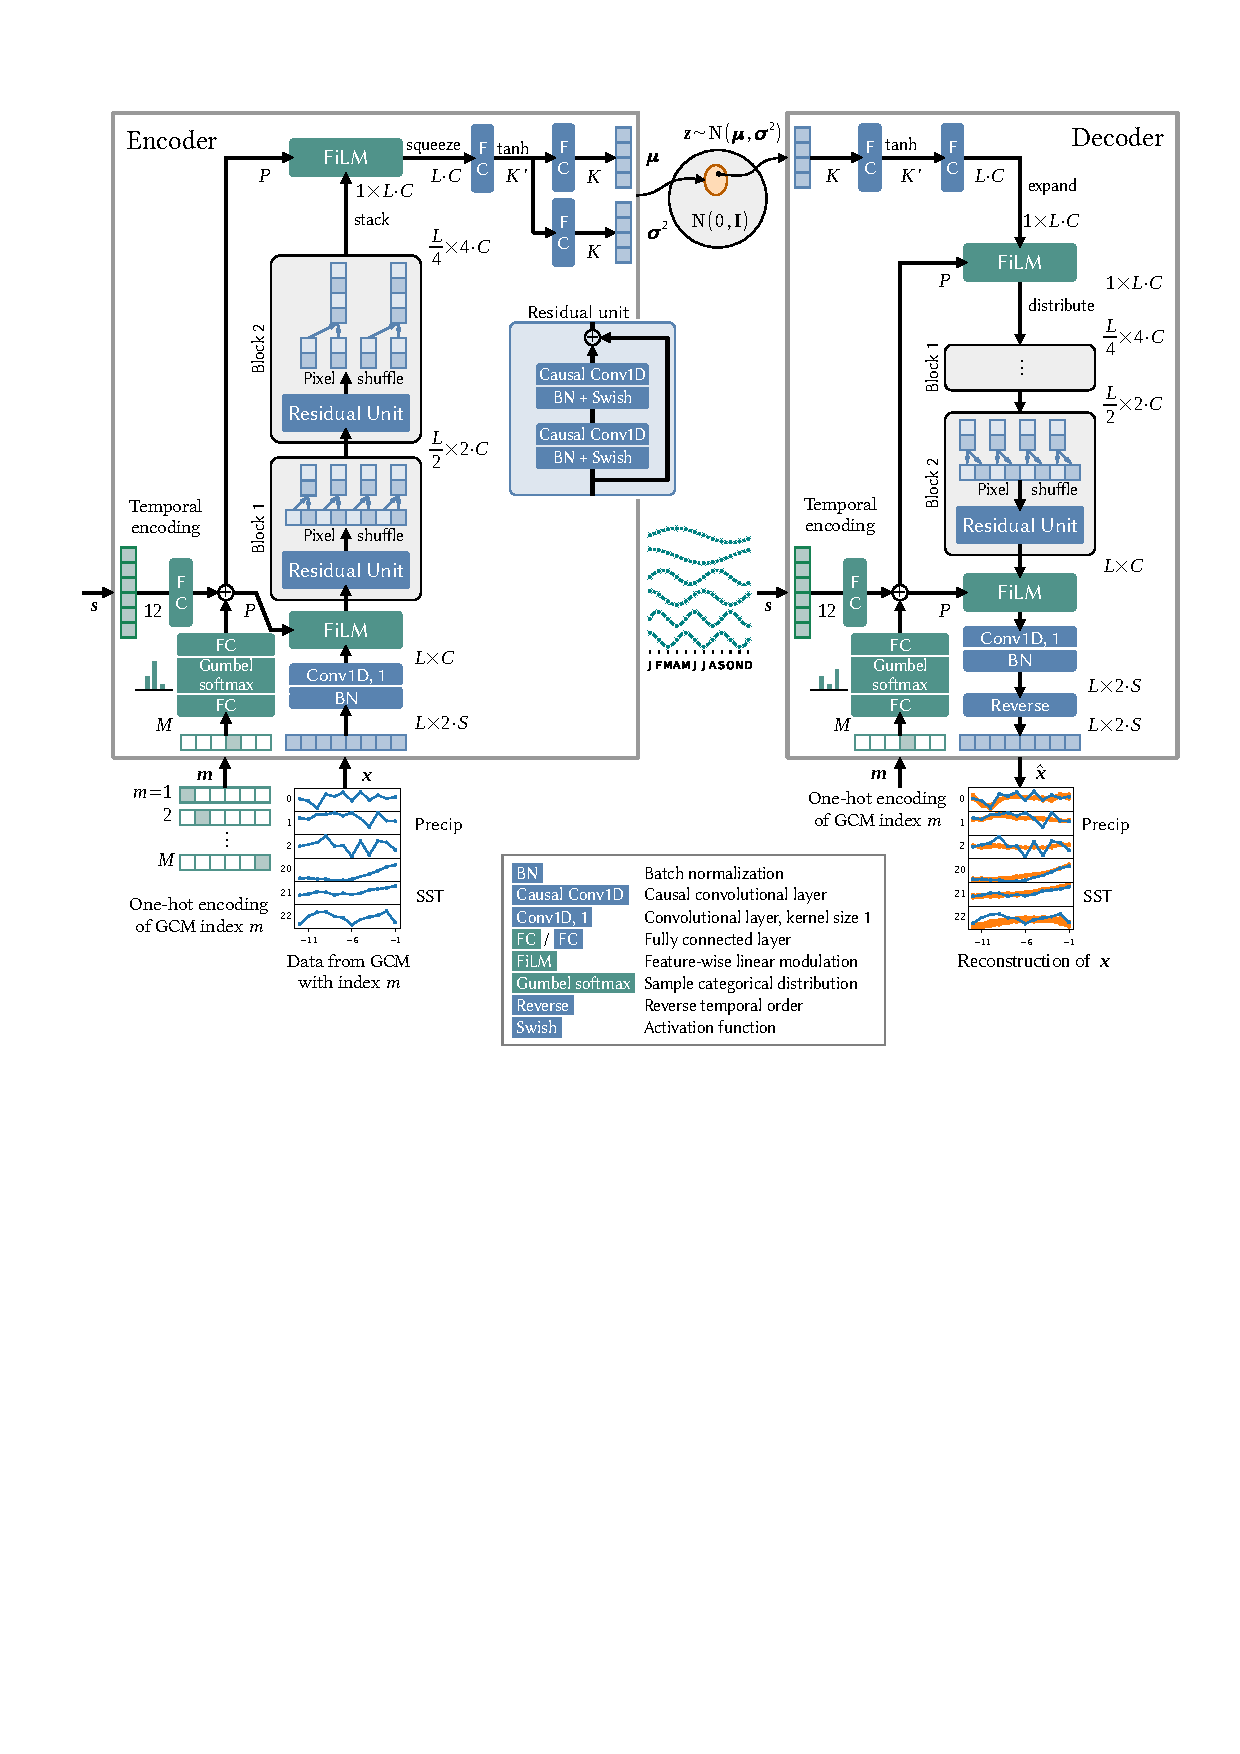
\includegraphics[width=\linewidth]{Fig2_model_details.pdf}
    \caption{\label{fig:model-details}Architecture of the encoder NN (left) and the decoder NN (right). The figure shows the case of $B=2$ blocks. Examples of the input data $\mathbf{x}$ to the encoder and the decoder output $\mathbf{\hat{x}}$ are shown below the corresponding parts. The encoder and decoder consist of multiple blocks combining causal convolutional layers and resampling layers (blue boxes) to aggregate and distribute temporal information. The one-hot encoded GCM index $\mathbf{m}$ and the temporal information $\mathbf{s}$ are used to modify intermediate features in the encoder and decoder NNs by FiLM layers (green boxes). Only the first decoder NN for reconstruction is shown, cf. Fig.~\ref{fig:model-overview}. The second decoder NN used for forecasting (not shown here) has the same structure and keeps the temporal order, i.e. has no reverse layer.}
\end{figure}

The following section provides a summary of the implementation details of the encoding and decoding NNs as introduced in \cite{Groth.Chavez.2023}; cf. also Fig.~\ref{fig:model-details}.

Both the encoder and decoder are implemented as residual networks \citep{He.Zhang.ea.2016} that process their input through a stack of \emph{residual units}. The output of a residual unit $f_{l}$ is combined with the input $x_{l}$ to the unit, $x_{l+1}=f_{l}(x_{l})+x_{l}$ which improves signal propagation from one unit to another. The residual units use full pre-activation \citep{He.Zhang.ea.2016a} in which the convolutional layers are preceded by a batch-normalization layer and the activation function. For the latter, we use the sigmoid linear unit or SiLU, a specific case of the swish activation function.

The convolutional layers use causal convolutions to ensure that temporal dependencies are modeled in the right order. However, by reversing the temporal order in the output of the decoder, the temporal dependencies are decoded in an anti-causal order. This way, the encoding and decoding NNs model the temporal dynamics in opposite direction: the encoder aggregates information in the data in the forward direction, which the decoder uses to model the data in the backward direction. In contrast, in the second decoding NN used for forecasting, the output is not reversed, so the prediction target $\mathbf{y}$ is modeled in the forward direction as shown in Fig.~\ref{fig:model-overview}.

To capture temporal dependencies on different time scales, the data is resampled in each of the $B$ residual blocks as shown in Fig.~\ref{fig:model-details}, i.e., sub-sampled at half the sampling rate in the encoder and up-sampled at twice the sampling rate in the decoder. To efficiently resample the data, a parameter-free variant of a pixel shuffling \citep{Shi.Caballero.ea.2016} is used in the implementation of \cite{Groth.Chavez.2023}. For some illustrative examples of the pixel-shuffle algorithm in the encoder and decoder see Fig.~\ref{fig:model-details}.

In the encoder, an initial convolutional layer with kernel size 1 embeds the input into an initial number of $C$ channels, which is used as input to the stack of $B$ residual blocks. The features that we extract from the stack are then used as input to a multilayer perceptron (MLP), from which we obtain the mean and variance of the posterior. In this MLP, we have a first fully-connected (FC) layer with $K'$ units and the hyperbolic tangent as nonlinearity, from which we obtain the mean and variance through a pair of FC layers with $K$ units each.

The two decoders in Fig.~\ref{fig:model-overview} are of the same structure, and we have omitted the second decoder in Fig.~\ref{fig:model-details}. Both decoders receive a sample from the latent space as input to an MLP, i.e., a pair of FC layers with $K'$ and $L\times C$ units, respectively, and with a hyperbolic tangent in the middle. The output of the MLP is then used as input to the stack of $B$ residual blocks, while a final convolutional layer with kernel size $1$ provides the desired number of output channels. The first decoder is used for reconstruction, and the second decoder is used for forecasting. Therefore, the first decoder reverses the temporal order of the data, while the second decoder keeps the temporal order.

\paragraph{Feature-wise linear modulation}
The computation in the stack of residual blocks is influenced by so-called FiLM layers that modify the computation in the residual blocks based on auxiliary conditioning information via a simple, Feature-wise Linear Modulation \citep[FiLM,][]{Perez.Strub.ea.2018}.

In \cite{Groth.Chavez.2023}, the VAE is conditioned on two types of information: a) temporal information on the current month and b) ensemble information on the current ensemble member.

To encode temporal information on the current month at time $t$, sine and cosine functions of different frequencies are combined,
\begin{equation}
    \mathbf{s}(t)=\left\{ \left(\sin(2\pi\frac{k}{12}t),\cos(2\pi\frac{k}{12}t)\right),\quad k=1,2,\dots,6\right\}.\label{eq:temporal-encoding}
\end{equation}
For illustration, the monthly values of the first six components of the temporal encoding are shown in Fig.~\ref{fig:model-details}. Provided as auxiliary input to the the VAE encoder and decoder, the temporal encoding allows them to seasonally adjust their computations.

To encode information about the current ensemble member $m$, a random number from a categorical distribution is drawn, where the different categories represent different members of the batch ensemble. As shown in Fig.~\ref{fig:model-details}, sampling from the categorical distribution is implemented by categorical reparameterization with Gumbel-Softmax \citep{Jang.Gu.ea.2017.Gumbel-softmax}, which allows the VAE to make the sampling process itself dependent on auxiliary information. Conditioning on the ensemble member index $m$ allows the encoder and decoder to learn a distribution of the feature-wise scale and bias parameters in the FiLM layers that are specific to each of the $M$ CMIP models.

\section{Model configuration and training}\label{app:model-params-training}

A summary of the exact values of the different model parameters of the VAE can be found in Table \ref{tab:model-params}. In total, the VAE has about 621\,k trainable parameters.
\begin{table}
    \caption{\label{tab:model-params}Summary of model configurations of encoder, decoder NNs as described in section~\ref{sec:model-architecture} and shown in Figs.~\ref{fig:model-overview} and \ref{fig:model-details}.}
    \centering{}
    \begin{tabular}{lcc}
        \toprule
        Parameter                  &             & Value        \\
        \midrule
        \# of input channels (PCs) & $2 \cdot S$ & $2 \cdot 20$ \\
        Input length (month)       & $L$         & 12           \\
        Prediction length (month)  & $F$         & 12           \\
        Embedding channels         & $C$         & 64           \\
        Residual blocks            & $B$         & 2            \\
        FC units                   & $K'$        & 96           \\
        Latent dimensions          & $K$         & 32           \\
        Size of batch ensemble     & $E$         & 6            \\
        Size of condition          & $P$         & 12           \\
        \midrule
        \# of model weights        &             & 621\,k       \\
        \bottomrule
    \end{tabular}
\end{table}

The VAE is first trained on a large dataset of CMIP6 data, cf. Section~\ref{sec:data}, which is used to initialize the weights of the encoder and the two decoders. During transfer learning, most of the weights of the encoder and decoders are kept fixed, and only a subset of the weights is updated when continue training on a smaller dataset of historical observations, cf. again Section~\ref{sec:data}.

We have tested various options of the transfer learning procedure, and robust results were obtained when we only updated the weights of the BN layers and the FC layers that provide the auxiliary information to the FiLM layers in the encoder and decoders. On the other hand, the weights of the residual blocks, the actually FiLM layers and the MLPs are kept fixed. In this way, the encoder and decoders learn to adapt the distribution of the latent space to the new dataset, while the residual blocks keep the temporal dynamics of the latent space fixed. This way, the VAE can be trained on a small dataset of historical observations, while the latent space is still informed by the large dataset of CMIP6 data.

In contrast, we have found that fine-tuning the weights of the residual blocks leads to overfitting, which is why we only fine-tune the weights of the BN layers and the FC layers that provide the auxiliary information to the FiLM layers in the encoder and decoders.

The transfer learning procedure is inspired by \cite{Wen.Tran.ea.2020}, who have shown life-long learning of neural networks with batch ensembles. Instead of updating all weights of the NN, only a subset of the weights is updated that modulates the computation of the NN.

The training configuration is summarized in table \ref{tab:model-training}. The model weights are optimized using the Adam optimizer \citep{Kingma.Ba.2014} and a fixed learning rate $l_r$. They are optimized on the objective in Eq.~\eqref{eq:total-loss} with stochastic gradient descend on mini-batches of size $N_{\mathcal{M}}$. The mini-batches are augmented with $r$ different members sampled from the batch ensemble so that the different members are jointly optimized on the same data. The training is performed in two stages. First, the model is trained on the enitre dataset of CMIP6 data for 10 epochs with a learning rate $l_r=1 \cdot 10^{-3}$. Then, the model is trained on the historical observations over the 1891--1980 period for 100 epochs with a learning rate $l_r=2 \cdot 10^{-4}$.

Since there is no index $m$ associated with the observations, the index $m$ is drawn randomly between $1\dots M$, where $M$ is the number of CMIP6 models. During the transfer learning, we found it beneficial to set the scale of the TC loss to a negative value, which means that the sign of the TC loss is flipped. This will lead to a maximization of the TC loss instead of a minimization. Since the model is given the same input for all batch ensemble members, the TC is maximized when the sampling from the Gumbel-Softmax becomes independent of the index $m$. During pre-training, conditioning on the index $m$ allows the VAE to learn a distribution of the feature-wise scale and bias parameters in the FiLM layers that are specific to each of the $M$ CMIP models. During transfer learning, the VAE is encouraged to learn a distribution of the feature-wise scale and bias parameters that is independent of the index $m$ and particular optimal for the historical observations.

\begin{table}
    \caption{\label{tab:model-training}Overview of the training configuration used in stochastic gradient descent and the corresponding scale parameters of the different loss terms in Eq.~\eqref{eq:total-loss}.}
    \centering{}
    \begin{tabular}{lccc}
        \toprule
        Parameter                    &                          & pre-training      & transfer learning \\
        \midrule
        Dataset                      &                          & CMIP6             & historical        \\
        Time period                  &                          & 1850--2014        & 1891--1980        \\
        \# training samples          &                          & 140\,k            & 1053              \\
        \# of trained model weights  &                          & 621\,k            & 4\,k              \\
        Batch size                   & $N_{\mathcal{M}}$        & 128               & 32                \\
        Ensemble members in batch    & $r$                      & 5                 & 5                 \\
        Augmented batch size         & $r\cdot N_{\mathcal{M}}$ & 640               & 160               \\
        Learning rate                & $l_r$                    & $1 \cdot 10^{-3}$ & $2 \cdot 10^{-4}$ \\
        Epochs                       &                          & 10                & 100               \\
        \midrule
        Scale of regularization      & $\beta$                  & $0\rightarrow5$   & 5                 \\
        Scale of TC term             & $\gamma$                 & 7                 & -1                \\
        Scale of CE term in decoder  & $\delta_{x}$             & 1                 & 1                 \\
        Scale of CE term in forecast & $\delta_{y}$             & 3                 & 1                 \\
        Scale of prediction loss     & $\alpha$                 & 3                 & 1                 \\
        \bottomrule
    \end{tabular}
\end{table}

\section{Results}\label{sec:results}
This section presents first results of the VAE model and the prediction of precipitation for the crop season several month ahead. We consider the crop season of soybean which is taken from the GGCMI crop calendar Phase 3 dataset \citep{Jaegermeyr.Mueller.ea.2021}.

\begin{figure}
    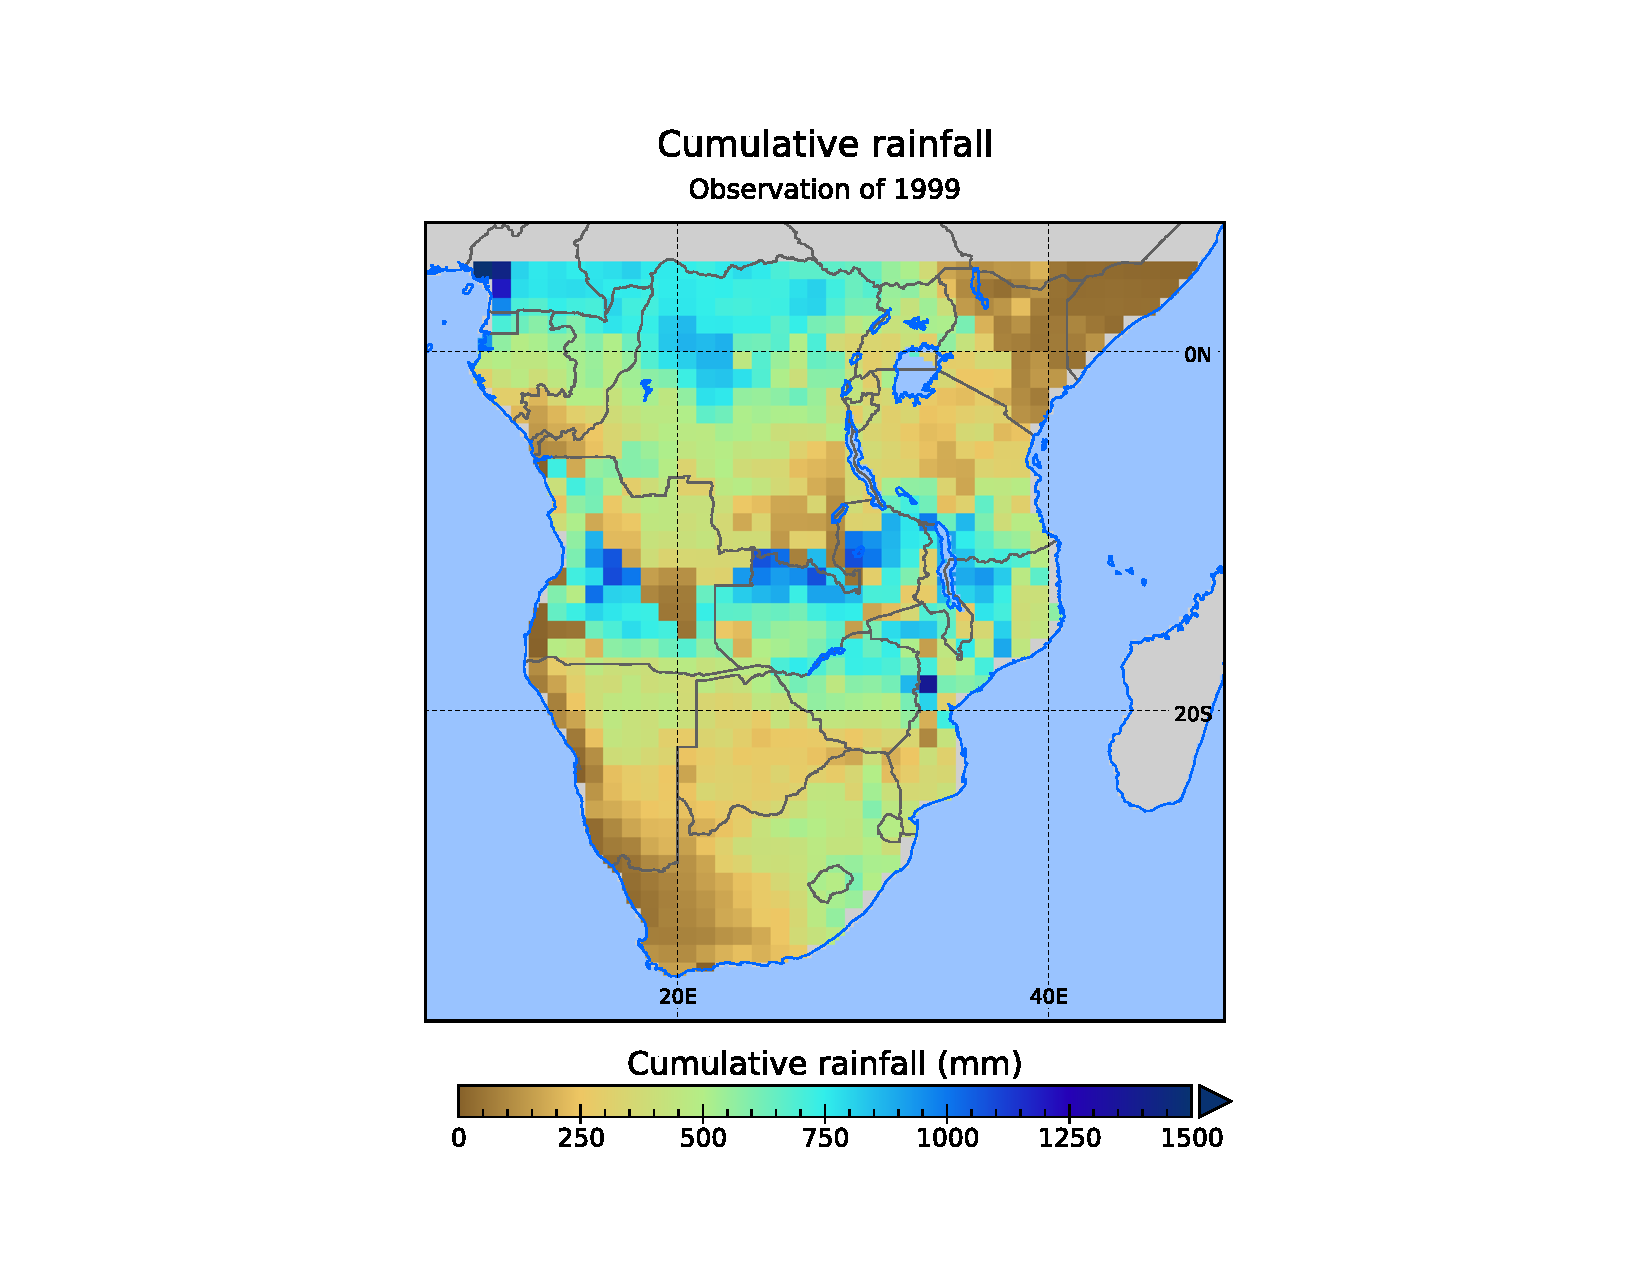
\includegraphics[width=0.32 \textwidth]{cum_precip.ensmedian.lag-1}
    \hfill
    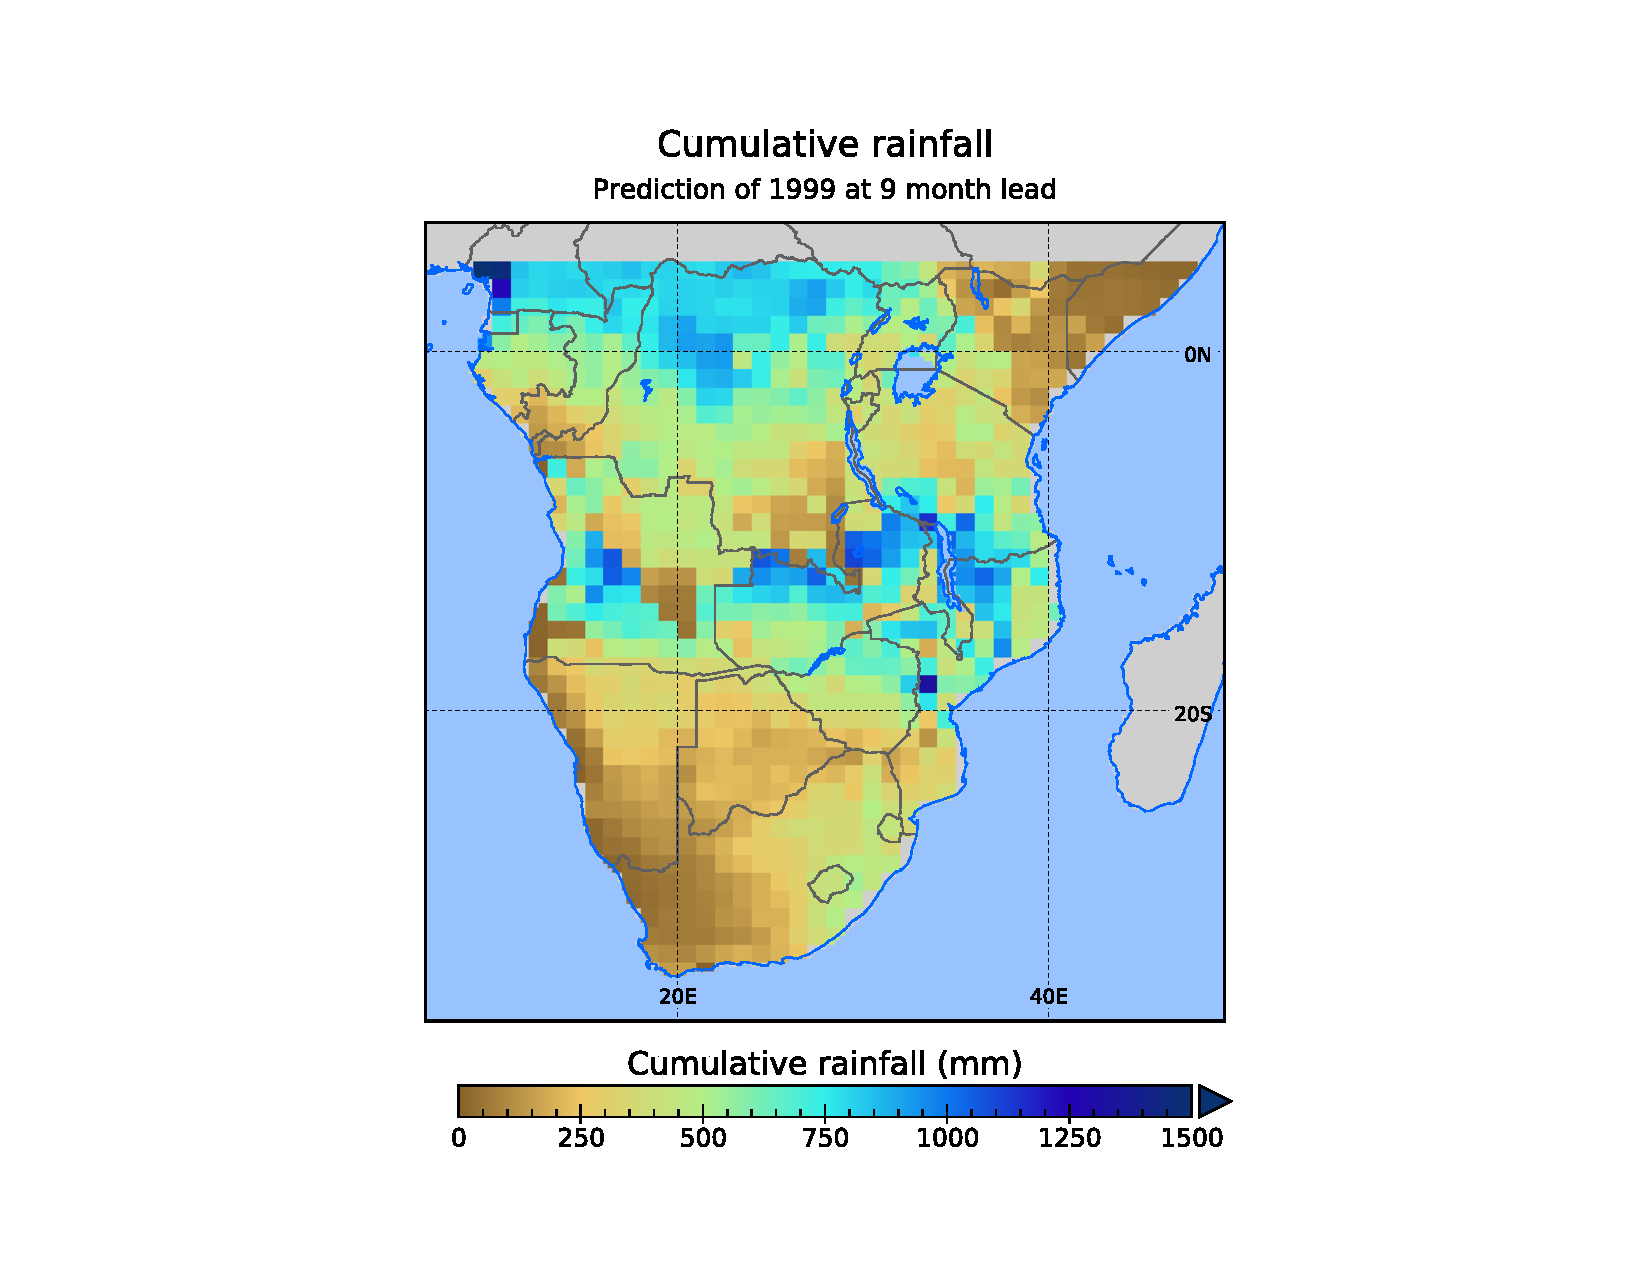
\includegraphics[width=0.32 \textwidth]{cum_precip.ensmedian.lag+8}
    \hfill
    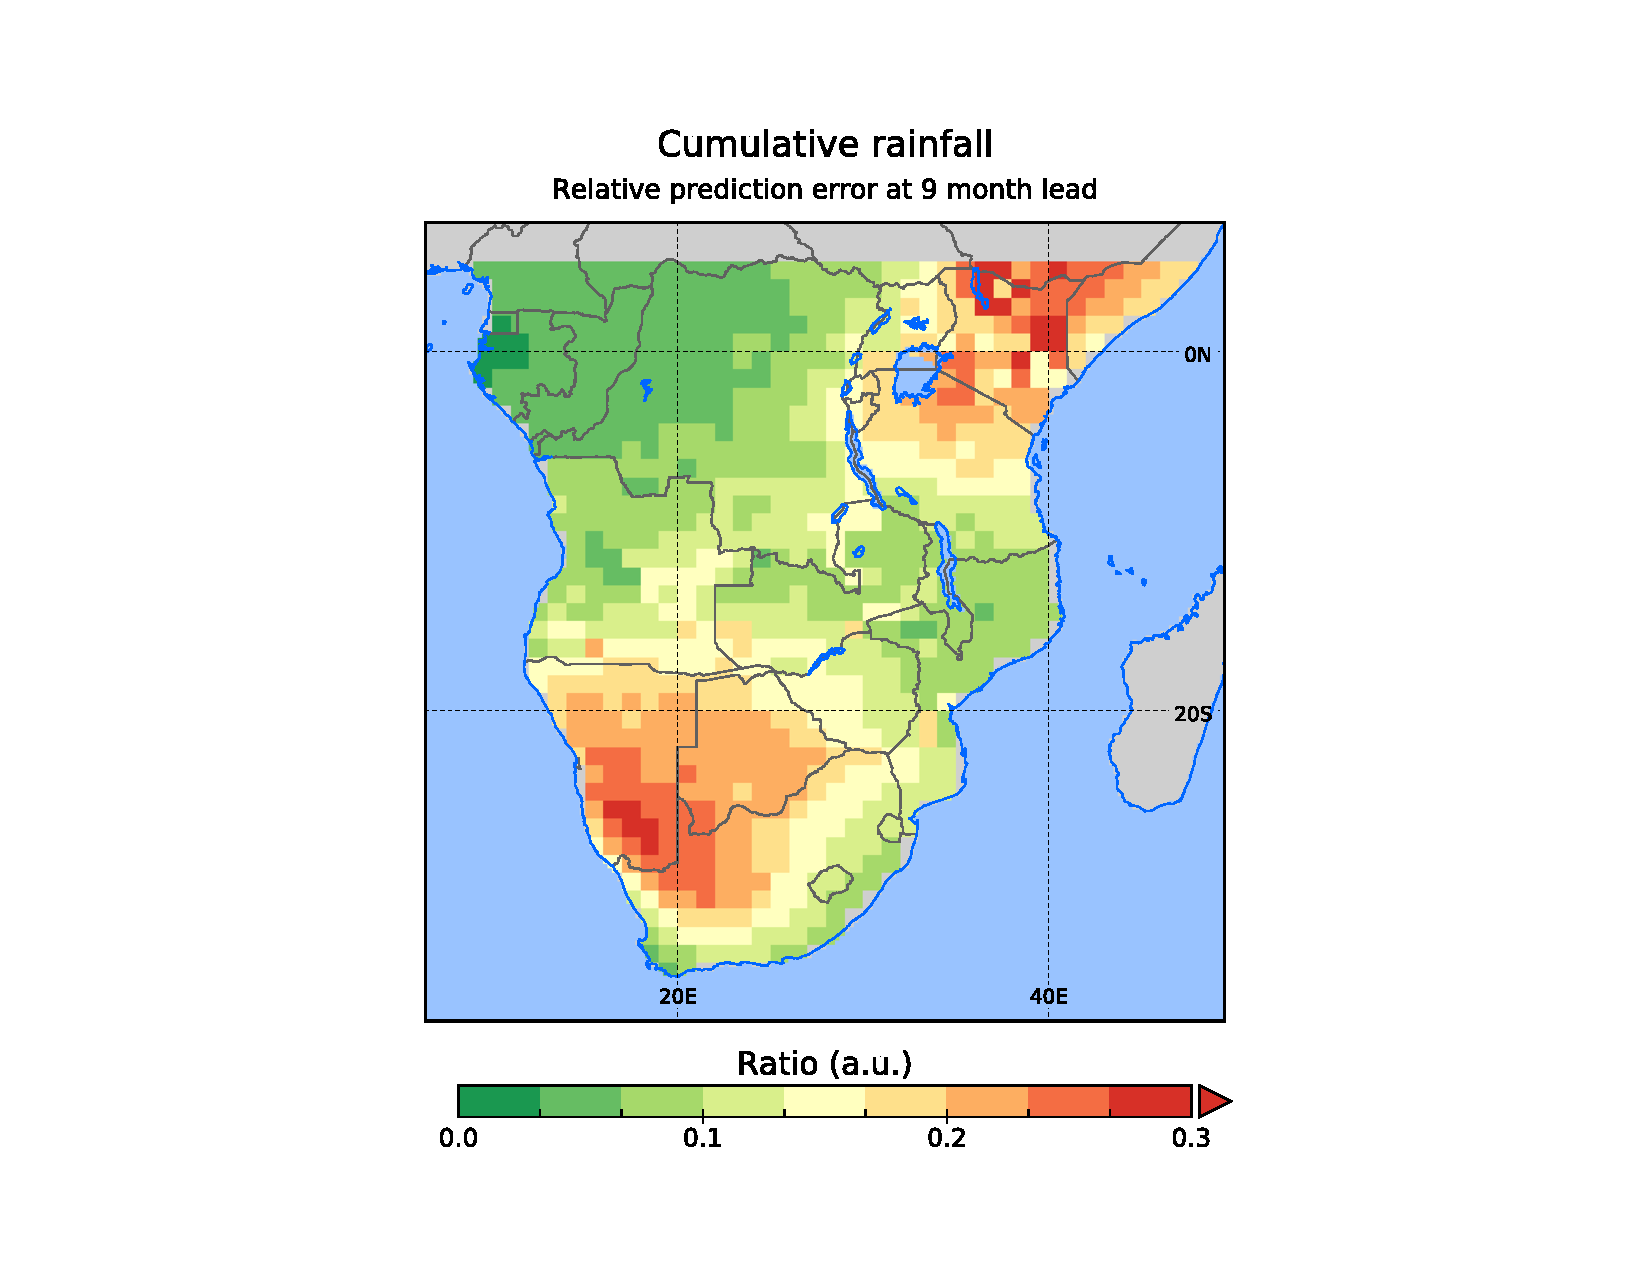
\includegraphics[width=0.32 \textwidth]{cum_precip.ensmedian.lag+8.rmae}
    \caption{\label{fig:precip-prediction-map}
        Map of cumulative rainfall for the crop season of soybean in the year 1999. Left: observed rainfall. Middle: predicted rainfall at 9 month lead time. Right: relative mean absolute error (RMAE) of the prediction over the crop seasons in the 1980--2019 period. The RMAE is defined as the mean absolute error of the prediction divided by the mean of the observed rainfall. Dates for the crop season taken from the GGCMI crop calendar Phase 3 dataset \citep{Jaegermeyr.Mueller.ea.2021}.}
\end{figure}
In Fig.~\ref{fig:precip-prediction-map}, we show the predicted rainfall for the crop season in the year 1999 and compare the prediction with the observed rainfall. The prediction is made at a lead time of 9 months for the crop season in the year 1999. We see that the VAE prediction provides a good estimate of the observed rainfall. The VAE prediction is able to capture the spatial distribution of the rainfall, and the predicted rainfall is in the same order of magnitude as the observed rainfall. The relative mean absolute error (RMAE) of the prediction is shown in the right panel of Fig.~\ref{fig:precip-prediction-map}. The RMAE is defined as the mean absolute error of the prediction divided by the mean of the observed rainfall. The RMAE is less than 0.2 for many of the regions in Africa, which means that the prediction error is less than 20\% of the mean rainfall. The RMAE is generally larger in regions with low rainfall, which is expected since the prediction error is relative to the mean rainfall.

\begin{figure}
    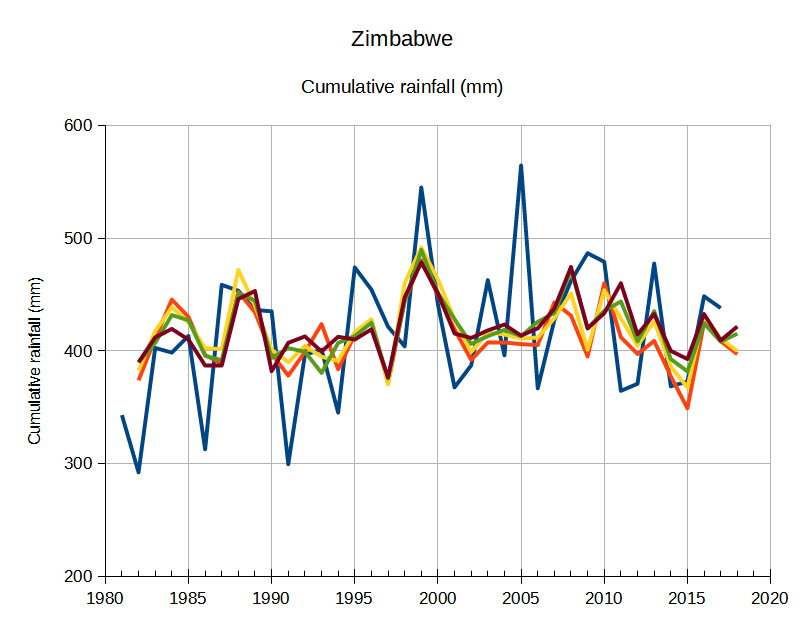
\includegraphics[height=5.4cm]{cum_precip.ensmedian.ZW}
    \hfill
    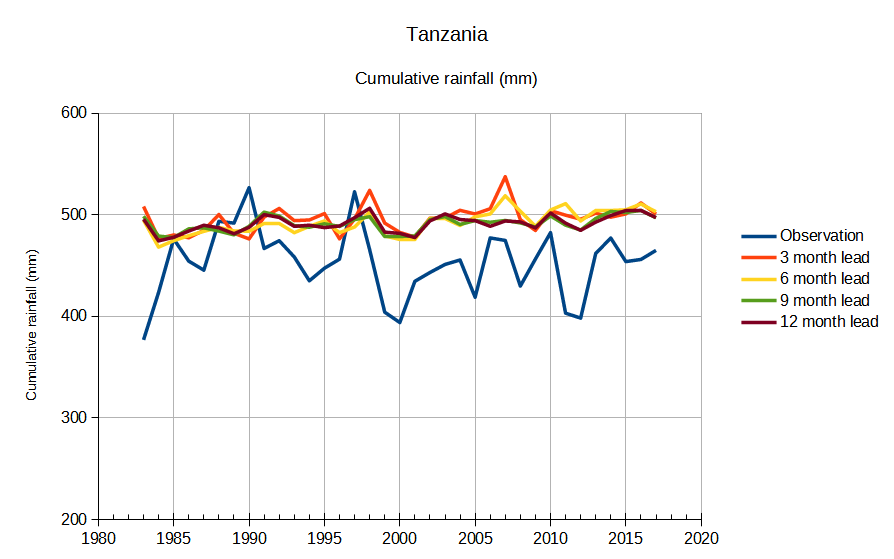
\includegraphics[height=5.4cm]{cum_precip.ensmedian.TZ}
    \caption{\label{fig:precip-prediction-country}
        Country average of cumulative rainfall for the crop seasons from 1980 to 2017. Left: Zimbabwe. Right: Tanzania. The plot compares the observed rainfall (blue) with the predicted rainfall at different lead times.}
\end{figure}
Next, we obtain the country averages of the predicted rainfall and compare them with the observed rainfall. The country averages obtained for Zimbabwe and Tanzania are shown in Fig.~\ref{fig:precip-prediction-country}. The VAE prediction is able to capture the observed rainfall particularly well in Zimbabwe. The prediction is made at different lead times, and we see that the prediction quality is quite constant with increasing lead time up to 12 month lead time. The prediction quality is less good for Tanzania than for Zimbabwe. To which extend the rainfall in Zimbabwe is more predictable than the rainfall in Tanzania is an interesting question that we will investigate in future work.

The overall picture of these results clearly demonstrates that the VAE model is able to predict the cumulative rainfall for the crop seasons in African countries at a lead time of 12 months. Since the VAE model has been trained on historical observations prior to 1980, the predictions made for the crop seasons in the 1980--2019 period represent the prediction skill of the VAE model for out-of-sample data.

\section*{Declarations}
\paragraph{Data and code availability}

The data and the Python scripts developed allowing to reproduce the experiments illustrated in this report are available at \url{https://github.com/andr-groth/VAE-precip-predict}.

\bibliographystyle{ametsoc2014}
\bibliography{VAE-precip-predict-biblio}


\end{document}
